% Which command writes which file, from training to a macro in the paper.
% Compiled by render.py.
\documentclass[tikz,border=6pt]{standalone}
\usepackage[T1]{fontenc}
\usepackage{lmodern}
\usetikzlibrary{arrows.meta,positioning,calc}

\definecolor{cmd}{HTML}{0072B2}
\definecolor{gpu}{HTML}{D55E00}
\definecolor{boxfill}{HTML}{F2F2F2}

\tikzset{
  file/.style={draw, fill=boxfill, font=\scriptsize\ttfamily, align=center,
    minimum height=11mm, text width=40mm},
  flow/.style={-{Stealth[length=1.6mm]}, thick},
  cmdlab/.style={font=\scriptsize\ttfamily, text=cmd, align=center},
  gpulab/.style={font=\scriptsize\ttfamily\bfseries, text=gpu, align=center},
}

\begin{document}
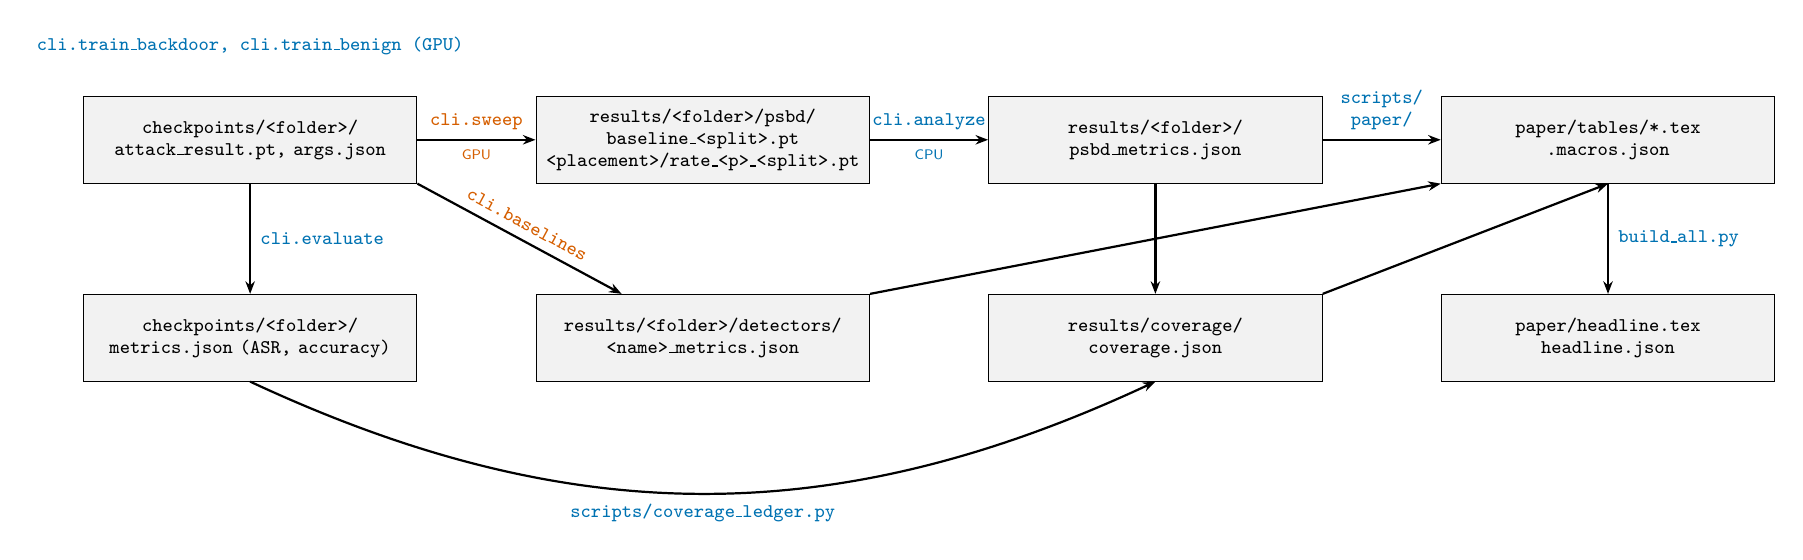
\begin{tikzpicture}[node distance=5mm and 15mm]

\node[file] (ckpt) {checkpoints/<folder>/\\attack\_result.pt, args.json};
\node[file, right=of ckpt] (cache) {results/<folder>/psbd/\\baseline\_<split>.pt\\<placement>/rate\_<p>\_<split>.pt};
\node[file, right=of cache] (metrics) {results/<folder>/\\psbd\_metrics.json};
\node[file, below=14mm of metrics] (ledger) {results/coverage/\\coverage.json};
\node[file, right=of metrics] (tables) {paper/tables/*.tex\\*.macros.json};
\node[file, below=14mm of tables] (headline) {paper/headline.tex\\headline.json};
\node[file, below=14mm of ckpt] (evalm) {checkpoints/<folder>/\\metrics.json (ASR, accuracy)};
\node[file, below=14mm of cache] (det) {results/<folder>/detectors/\\<name>\_metrics.json};

\draw[flow] (ckpt) -- node[above, gpulab] {cli.sweep} node[below, font=\tiny\sffamily, text=gpu] {GPU} (cache);
\draw[flow] (cache) -- node[above, cmdlab] {cli.analyze} node[below, font=\tiny\sffamily, text=cmd] {CPU} (metrics);
\draw[flow] (metrics) -- node[above, cmdlab] {scripts/\\paper/} (tables);
\draw[flow] (tables) -- node[right, cmdlab] {build\_all.py} (headline);
\draw[flow] (ckpt) -- node[right, cmdlab] {cli.evaluate} (evalm);
\draw[flow] (ckpt.south east) -- node[above, sloped, gpulab] {cli.baselines} (det);
\draw[flow] (evalm.south) to[out=-25, in=-155] node[below, cmdlab, pos=0.5] {scripts/coverage\_ledger.py} (ledger.south);
\draw[flow] (metrics) -- (ledger);
\draw[flow] (ledger.north east) -- (tables.south);
\draw[flow] (det.north east) -- (tables.south west);

\node[above=4mm of ckpt, cmdlab] {cli.train\_backdoor, cli.train\_benign (GPU)};

\end{tikzpicture}
\end{document}
